\chapter{Statistical tests}
\label{ch:statistics}

%Explain which test used and why and how they work

%shapiro wilk
\section{Normal distribution}
When choosing a statistical test we have to take into consideration the preconditions for using the test. The most common precondition is that the data follows a normal distribution. The Shapiro-Wilk test has more power then the other normality tests \cite{razali2011power} and therefor this test was used. The Shapiro-Wilk test calculates a statistic by dividing the the summation to the power of two of every point times a coefficient by the summation of  every point minus the mean to to the power of two \cite{shapiro1965analysis}. This formula is shown in equation \ref{eq:sw}. The null-hypothesis of the Shapiro-Wilk test is that the data is normally distributed. This means that when the null-hypothesis gets rejected the data does not follow a normal distribution. For this test we used an \textit{alpha}-value of 0.01, because distributions that are close to normally distributed can still be used in some of the statistical tests. When testing if the energy measurements from a single program on a single node follow the normal distribution using the Shapiro-Wilk test we get that not all programs measurements are normally distributed. From the 269 different programs 183 were not normally distributed on node029 and 38 on node028. Therefor we need to choose statistical test that don't assume the data to be normally distributed.

\begin{equation}
    W = \frac{(\sum_{i=1}^{n} a_{i}x_{(i)})^2}{\sum_{i=1}^{n} (x_{i} - \bar x)^2}
    \label{eq:sw}
\end{equation}

%The data we want to test for normality is all the measurement points of one program on one machine.

\section{Same distribution}
%Kolmogorov–Smirnov test, Mann Whitney U test
When comparing different programs, that are in the same language and have the same functionality, we need to find out if there is a significant difference concerning the energy consumption. This can be tested by looking at the two different distributions and testing if they are from the same population. A statistical test that compares two distribution and test there equality is called the Mann Whitney U test \cite{mann1947test}. Here the null hypothesis is that the distributions are from the same population. The Mann Whitney U test looks if the chance that a random variable from the first distribution is greater than a random variable from the second distribution. When this chance is 50\%, then the two different distributions belong to the same population. Another test that we could have used was the students t-test. This test however has the preconditions that the means of the two distributions should follow the normal distribution and the variance of the two distributions should be equal. Our data doesn't match these precondition and therefor we chose to use the Mann Whitney U test.\\

There are two versions of the Mann Whitney U test, the one-sided and the two-sided test. For the two-sided Mann Whitney U test the alternative hypothesis is that the distributions are from the same population, but if you want to know the direction of this comparison you need to use the one-sided Mann Whitney test \cite{nachar2008mann}. Which means that the alternative hypothesis for the one-sided Mann Whitney U test is that the first distribution is stochastically larger than the second distribution \cite{nachar2008mann}. Because rejecting the null hypothesis holds more power than not rejecting the null hypothesis, a one-sided Mann Whitney U test was used twice. We tested if the first distribution was stochastically larger than the second distribution and if the second distribution was stochastically larger than the first, with an  \textit{alpha}-value of 0.05. If both these tests reject the null hypothesis then we still don't know for certain that the distributions are from the same population.\\

We also used the two sample Kolmogorov-Smirnov test to find out if two distributions are from the same population. This test also has as its null hypothesis that the two distributions are from the same population and we used an \textit{alpha}-value of 0.05. The Kolmogorov-Smirnov test compares the empirical distribution functions of the two distributions.

\section{Correlation}
%pearson, kendall tau, sampled and first removed why, 
A commonly known method for calculating the correlation is called the Pearson coefficient. The Pearson coefficient uses the covariance of two variables to calculate its correlation score \cite{pearson1929some}. For this method the following assumptions should hold, the correlation is linear and the data follows a normal distribution. Our data however does not meet these assumptions for all programs and therefor we needed to look at a different method. The Kendall Tau coefficient calculates a ranked correlation coefficient and does not assume that the data follows a normal distribution \cite{kendall1938new}, therefor this method was used. The Kendall Tau method looks at how many pairs of points follow the same order. For example points $(x_i, y_i)$ and $(x_j, y_j)$ follow the same order if $x_i > x_j$ and $y_i > y_j$ or if $x_i < x_j$ and $y_i < y_j$. Because every pair needs to be checked this could get computational heavy for large number of points, luckily that is not the case in this research project.\\

The coefficient is in the range of one to minus one, where at zero there is no correlation and at one or minus one there is. But what about the scores in between? According to the standard Guilford scale the range $0-0.2$ means slight correlation, $0.2-0.4$ means low correlation, $0.4-0.7$ means moderate correlation, $0.7-0.9$ means high correlation and $0.9-1$ means very high correlation \cite{guilford1950fundamental}. Because the minus in the coefficient shows which direction the correlation is in, we can use the absolute value to determine in which range of correlation a negative number is. 

\section{Anomaly detection}
%dbscan
An anomaly, also called outlier, is a point that does not behave like the rest of the points in the results. These anomalies can be detected by using a clustering algorithm like DBSCAN \cite{chandola2009anomaly}. The DBSCAN algorithm goes though every point and counts how many other points are in a predefined area around the point. If there are more or equal to the minimum amount of points needed in this area then this point is labelled as a core point. Points that are not core points but are in the predefined area around a core point are labelled border points, all the other points are anomalies \cite{ester1996density}. This is visualized in figure \ref{fig:dbscan}, where all red dots are core points, yellow dots border points and blue dots anomalies. The minimum amount of points needed around a point and the predefined area around a point are the input variables of this algorithm, which is the disadvantage of this method.

\begin{figure}[h]
    \centering
    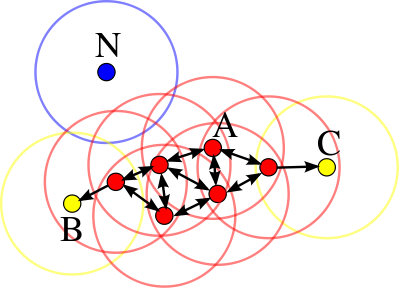
\includegraphics[width=.4\textwidth]{graphs/dbscan.png}
    \caption{The labels according to DBSCAN algorithm with minimum points is four, where the red dots are core points, yellow dots border points and blue dots anomalies. Core points are points that have within a certain distance a minimum amount of points. Border points don't have the minimum amount, but are within reach of a core point. Anomalies don't have the minimum amount of points in a certain area and are not reachable from a core point. (source: \url{https://en.wikipedia.org/wiki/DBSCAN})}
    \label{fig:dbscan}
\end{figure}

\subsection{Input variables}
%eps and minpts
According to \cite{ester1996density} we can set the minimum amount of points a core point needs in his area to four for two dimensional data. However for the area we need to calculate the radius, also called the eps variable. This eps is calculated by first calculating the distance to the fourth nearest neighbour for every point. These distances are then sorted and plotted. The value for eps can then be read from the graph looking at the first valley \cite{ester1996density}. In our implementation we calculated this eps automatically for every single program. To retrieve the first valley we looked at the differences between the slopes around a point. The point with the biggest difference in slopes was in the valley and was used as our eps variable for that specific program.\\

These two parameters have a big influences on how the clusters are divided and which points are labelled as an anomaly. When the minimum amount of points gets smaller more clusters will be formed and when it gets larger less clusters will be formed, assuming eps stays the same. When eps gets smaller more points will be labelled as anomalies and when eps get larger less points will be labelled as anomalies, assuming the minimum points parameter stays the same.

\section{Clustering}
%kmeans
When trying to find clusters in our data we were searching for a specific amount of clusters. Because the amount of clusters was known before clustering the k-means clustering algorithm was used. This algorithm begins by randomly assigning means for the amount of clusters specified. Then all the points are passed and divided into a cluster based on which mean has the shortest euclidean distance. After this the mean of the clusters is calculated and these will be the new means. This will iterate till a local maximum is found or the maximum amount of iterations has passed. The maximum amount of iterations was left to the default of 300 form the \textit{sklearn} python packages.